\chapter{The Recovery of the $M_{\rm BH} - n_{\rm sph}$ Relation}
\label{ch:recov-mn}

\cite{graham2001} demonstrated that the mass of SMBHs is correlated 
with the stellar light concentration of their host spheroid. 
Six years later, \cite{grahamdriver2007} expanded the galaxy sample of \cite{graham2001} 
and carried out 1D bulge/disc decompositions. 
They described the 1D surface brightness profile of spheroids with the S\'ersic model, 
and obtained a direct measure of the central radial concentration of stars 
by means of the S\'ersic index. 
\cite{grahamdriver2007} confirmed the early findings of \cite{graham2001}, 
presenting a strong correlation between the black hole mass and the spheroid S\'ersic index ($M_{\rm BH} - n_{\rm sph}$). 
They measured a small level of scatter, 
which made the $M_{\rm BH} - n_{\rm sph}$ and $M_{\rm BH} - \sigma_*$ correlations 
evenly competing for the title of fundamental black hole mass scaling relation. \\

As the number of directly measured black hole masses increased with time and
the constantly improving technology of machines allowed shorter computational times for 2D decomposition codes, 
more studies were dedicated to the analysis of various black hole mass scaling relations. 
\cite{sani2011}, \cite{vika2012}, and \cite{beifiori2012} attempted 2D decompositions 
of their samples of galaxies with a direct measure of the black hole mass. 
\citeauthor{sani2011} and \citeauthor{vika2012} included more than two components in their galaxy models 
such as bars and nuclear sources, 
whereas \citeauthor{beifiori2012} excluded barred galaxies from their analysis 
and used simple bulge+disc models. 
From these decompositions, they derived and analysed several correlations. 
However, none of these three studies was able to obtain a strong $M_{\rm BH} - n_{\rm sph}$ relation from their data. 
This raised an obvious question: 
what prevented \citeauthor{sani2011}, \citeauthor{vika2012}, and \citeauthor{beifiori2012} 
from the recovery of a tight $M_{\rm BH} - n_{\rm sph}$ correlation? 
Imputable factors could be the decomposition technique (1D versus 2D), 
the use of more sophisticated models featuring a larger number of components, 
the use of different wavelengths, 
or possibly the accuracy of the decompositions. \\

These circumstances motivated us to engage a preliminary study in 2012, 
aiming at explaining the lack of an $M_{\rm BH} - n_{\rm sph}$ correlation 
in the data of \citeauthor{sani2011}, \citeauthor{vika2012}, and \citeauthor{beifiori2012} 
After collecting and comparing the results from the galaxy decompositions 
of the aforementioned four studies (\citeauthor{grahamdriver2007}, \citeauthor{sani2011}, 
\citeauthor{vika2012}, and \citeauthor{beifiori2012}), 
we immediately noticed that some galaxies had been described by these authors with significantly different models 
(e.g.~the galaxy M60, treated as a discless elliptical galaxy by two studies, 
and as a lenticular galaxy by the other two studies). 
Different galaxy models (for the same galaxy) evidently resulted in different best-fit parameters. 
Not only this, but some studies obtained largely discrepant best-fit parameters 
for the same galaxy even when they used the same choice of decomposition 
(e.g.~two studies described the galaxy NGC 3115 with a S\'ersic-bulge + exponential-disc model, 
but obtained a bulge S\'ersic index of $3$ and $13$, respectively). 
This confirmed our doubts about the accuracy of some decompositions. \\

For each galaxy, we averaged the available S\'ersic index measurements 
and used these average values to populate the $M_{\rm BH} - n_{\rm sph}$ diagram. 
We noticed that a clear correlation was emerging from the data, 
although with a significant amount of scatter. 
We attributed the large amount of scatter to ``bad'' decompositions, 
and decided to develop a method for an impartial identification of the ``bad'' S\'ersic index measurements. 
After estimating a maximum tolerable disagreement between the S\'ersic index measurements of the same galaxy 
by taking into account the use of different decomposition methods and wavelengths, 
we excluded the most discrepant measurements and averaged the remaining ones. 
This resulted in a dramatic reduction of scatter 
and the recovery of a strong $M_{\rm BH} - n_{\rm sph}$ correlation. 
Finally, we explored substructure in the $M_{\rm BH} - n_{\rm sph}$ diagram 
expected for consistency with other known scaling relations. \\

The remainder of this Chapter comprises the published version of the paper 
``The supermassive black hole mass -- S\'ersic index relations for bulges and elliptical galaxies''
by G.~A.~D.~Savorgnan et al., 
as it appears in Volume 434 of \emph{Monthly Notices of the Royal Astronomical Society}. 


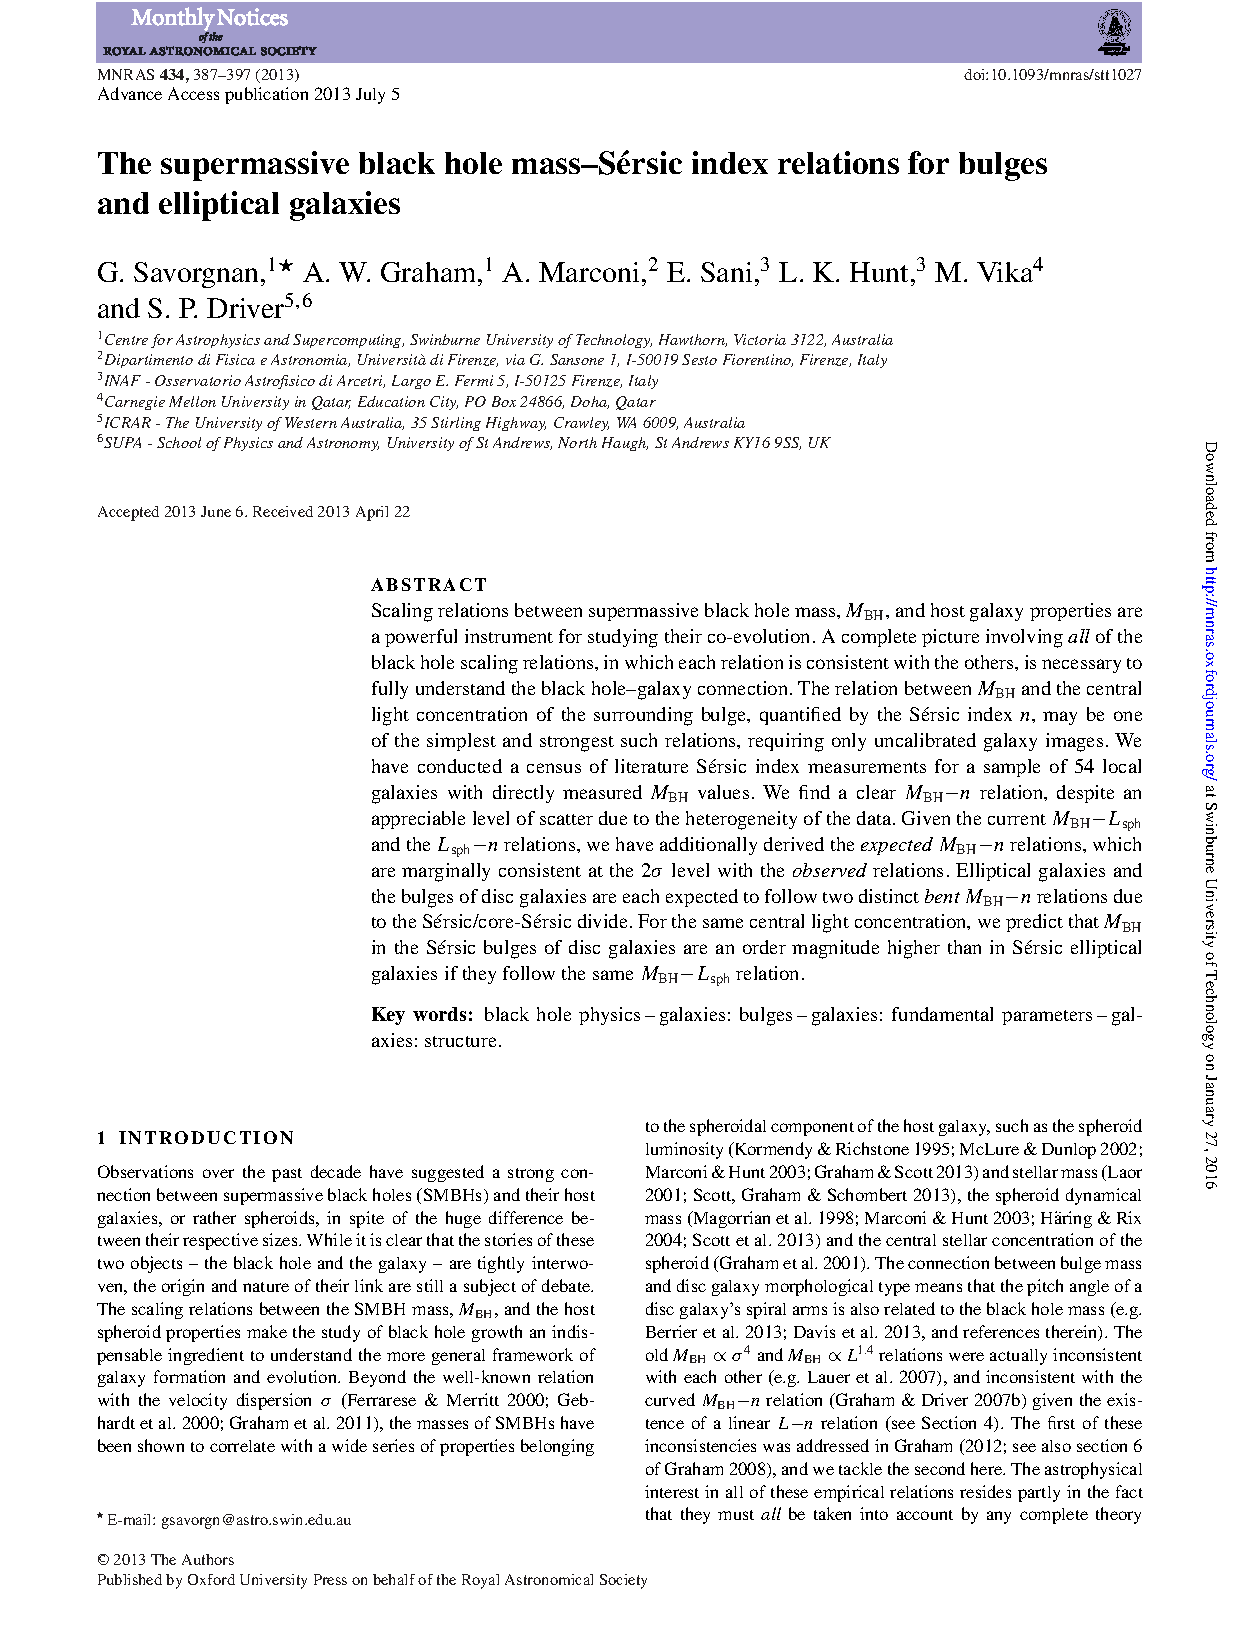
\includepdf[pages={1-11}]{MNRAS2013.pdf}
